\documentclass[]{standalone}
%\documentclass[dvisvgm]{minimal}

\usepackage[]{tikz}
\usepackage{sfmath}
\usepackage{pgfplots}
\pgfplotsset{compat=1.16}

\usetikzlibrary {positioning}

\renewcommand{\familydefault}{\sfdefault}

\definecolor{utorange}{rgb}{0.8,0.33,0.}
\definecolor{darkgreen}{rgb}{0.25,0.65,0.10}
\definecolor{darkblue}{rgb}{0,0,0.7}
\definecolor{MitRed}{RGB}{163, 31, 52}

\begin{document}
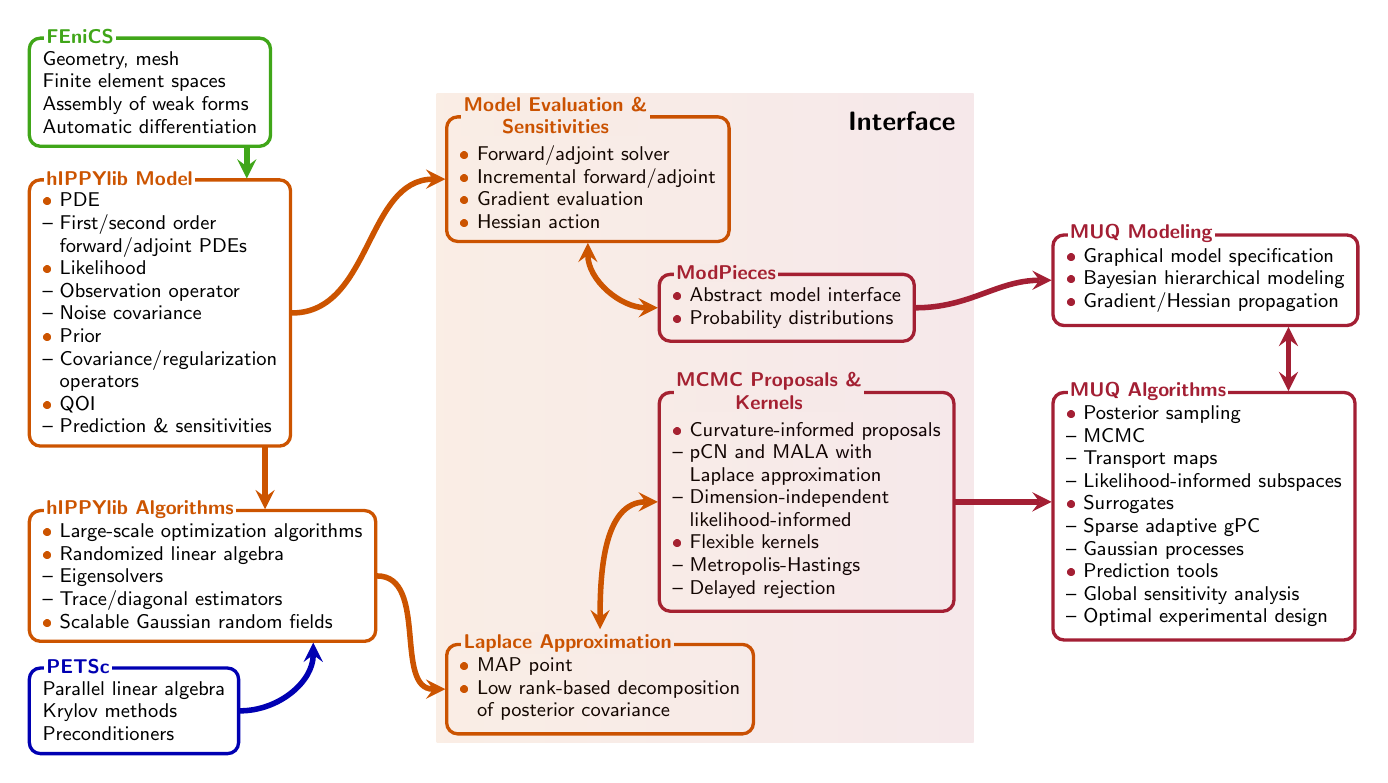
\begin{tikzpicture}[->, >=stealth, line width=0.2em,
  every node/.style={font=\fontsize{9}{10.2}\selectfont, scale=0.8}]
  \def\mybox#1#2#3#4#5{
    \node[draw=#1, very thick, rounded corners,
    anchor=north west, inner sep=6, align=left]
    (#2) at #3 {#4};
    \node[#1, inner sep=1, fill=white,
    anchor=west, right=0.5em, align=center] at (#2.north west) {#5};
  }
  %\draw[help lines] (0,0) grid (16,9);

  \mybox{darkgreen}{fenics}{(0,9)}
  {Geometry, mesh\\
    Finite element spaces\\
    Assembly of weak forms\\
  Automatic differentiation}
  {\textbf{FEniCS}}

  \mybox{utorange}{hlmodel}{(0,7.2)}
  {\textcolor{utorange}{\textbullet} PDE\\
    -- First/second order\\
    \phantom{--} forward/adjoint PDEs\\
    \textcolor{utorange}{\textbullet} Likelihood\\
    -- Observation operator\\
    -- Noise covariance\\
    \textcolor{utorange}{\textbullet} Prior\\
    -- Covariance/regularization\\
    \phantom{--} operators\\
    \textcolor{utorange}{\textbullet} QOI\\
    -- Prediction \& sensitivities
  }
  {\textbf{hIPPYlib Model}}

  \mybox{utorange}{hlalgorithms}{(0,3)}
  {\textcolor{utorange}{\textbullet} Large-scale optimization algorithms\\
    \textcolor{utorange}{\textbullet} Randomized linear algebra\\
    -- Eigensolvers\\
    -- Trace/diagonal estimators\\
  \textcolor{utorange}{\textbullet} Scalable Gaussian random fields}
  {\textbf{hIPPYlib Algorithms}}

  \mybox{darkblue}{petsc}{(0,1)}
  {Parallel linear algebra\\ Krylov methods\\ Preconditioners}
  {\textbf{PETSc}}

  \mybox{utorange}{hloutputs1}{(5.3,8)}
  {\phantom{\tiny phantom}\\
    \textcolor{utorange}{\textbullet} Forward/adjoint solver\\
    \textcolor{utorange}{\textbullet} Incremental forward/adjoint\\
    \textcolor{utorange}{\textbullet} Gradient evaluation\\
  \textcolor{utorange}{\textbullet} Hessian action}
  {\textbf{Model Evaluation \&}\\ \textbf{Sensitivities}}

  \mybox{utorange}{hloutputs2}{(5.3,1.3)}
  {
    \textcolor{utorange}{\textbullet} MAP point\\
    \textcolor{utorange}{\textbullet} Low rank-based decomposition\\
  \phantom{\textcolor{utorange}{\textbullet}} of posterior covariance}
  {\textbf{Laplace Approximation}}

  \mybox{MitRed}{muqmodpieces}{(8,6)}
  {\textcolor{MitRed}{\textbullet} Abstract model interface\\
  \textcolor{MitRed}{\textbullet} Probability distributions}{\textbf{ModPieces}}

  \mybox{MitRed}{muqmcmc}{(8,4.5)}
  {\phantom{\tiny phantom}\\
    \textcolor{MitRed}{\textbullet} Curvature-informed proposals\\
    -- pCN and MALA with\\
    \phantom{--} Laplace approximation\\
    -- Dimension-independent\\
    \phantom{--} likelihood-informed\\
    \textcolor{MitRed}{\textbullet} Flexible kernels\\
    -- Metropolis-Hastings\\
    -- Delayed rejection
  }
  {\textbf{MCMC Proposals \&}\\ \textbf{Kernels}}


  \mybox{MitRed}{muqmodeling}{(13,6.5)}
  {\textcolor{MitRed}{\textbullet} Graphical model specification\\
    \textcolor{MitRed}{\textbullet} Bayesian hierarchical modeling\\
  \textcolor{MitRed}{\textbullet} Gradient/Hessian propagation}
  {\textbf{MUQ Modeling}}

  \mybox{MitRed}{muqalgorithms}{(13,4.5)}
  {\textcolor{MitRed}{\textbullet} Posterior sampling\\
    -- MCMC\\
    -- Transport maps\\
    -- Likelihood-informed subspaces\\
    \textcolor{MitRed}{\textbullet}
    Surrogates\\
    -- Sparse adaptive gPC\\
    -- Gaussian processes\\
    \textcolor{MitRed}{\textbullet}
    Prediction tools\\
    -- Global sensitivity analysis\\
    -- Optimal experimental design
  }
  {\textbf{MUQ Algorithms}}

  \shade[opacity=0.1, right color=MitRed, left color=utorange]
  ([xshift=-8em, yshift=-4.7em] muqmcmc.south west) rectangle
  ([xshift=+2.1em, yshift=+6.5em] muqmodpieces.north east);
  \node[above] at ([xshift=-.5em, yshift=+4.8em] muqmodpieces.north east) {\large \textbf{Interface}};

  \path ([xshift=+3.5em] fenics.south) edge[darkgreen]
  ([xshift=+3.5em] fenics.south |- hlmodel.north)
  (petsc.east) edge[out=0, in=-90, darkblue] ([xshift=+4em] hlalgorithms.south)
  ([xshift=+3.8em] hlmodel.south) edge[utorange]
  ([xshift=+3.8em] hlmodel.south |- hlalgorithms.north)
  (hlmodel.east) edge[out=0, in=180, utorange] (hloutputs1.west)
  (hlalgorithms.east) edge[out=0, in=180, utorange] (hloutputs2.west)
  (hloutputs1.south) edge[<->, out=-90, in=180, utorange] (muqmodpieces.west)
  ([yshift=+0.5em] hloutputs2.north) edge[<->, out=90, in=180, utorange] (muqmcmc.west)
  (muqmodpieces.east) edge[out=0, in=180, MitRed]
  (muqmodeling.west)
  (muqmcmc.east) edge[MitRed] (muqmcmc.east -| muqalgorithms.west)
  ([xshift=+3em]muqmodeling.south) edge[<->, MitRed]
  ([xshift=+3em]muqmodeling.south |- muqalgorithms.north);
\end{tikzpicture}
\end{document}


